\documentclass[11pt,letter]{article}
\usepackage[top=1.00in, bottom=1.0in, left=1.1in, right=1.1in]{geometry}
\renewcommand{\baselinestretch}{1.1}
\usepackage{graphicx}
\usepackage{natbib}
\usepackage{amsmath}

\def\labelitemi{--}
\parindent=0pt

\usepackage[
singlelinecheck=false % <-- important
]{caption}
\usepackage{float}
\usepackage{hyperref}

\begin{document}
\bibliographystyle{/Users/Lizzie/Documents/EndnoteRelated/Bibtex/styles/besjournals}
\renewcommand{\refname}{\CHead{}}

\title{Safety plan for Wolkovich Lab: Okanagan field work}
\date{\today}
% \author{}
\maketitle
\tableofcontents

\section{Personnel, Contact Information and Safety Training}

\subsection {Feild Crew}

There will be a main team of two feild operatives (Faith Jones and Mira Garner) for the full three week period, and and additional feild crew member (Elizabeth Wolkovich) for the first week. Faith and Mira will travel up in one vehicle (\textbf{\textit{insert vehicle licence plate}}), and Elizabeth in another other (\textbf{\textit{insert licence plate}}). Elizabath will also stay at a different location to Faith and Mira, although both locations will be within (\textbf{\textit{x}} km from Kelowna.   

\subsection {Conact Details}

\begin{table}[H]
\caption{Feild crew contact details} % title of Table
%\centering % used for centering table. I dont want my tabel centred 
\begin{tabular}{ l | l }  % left jusitfy columns (2 columns)
\hline\hline %inserts double horizontal lines
Name & Contact\\ [0.5ex] % inserts table
%heading
\hline % inserts single horizontal line
Elizabeth Wolkovich & ? \\ % inserting body of the table
Faith Jones & 604 786 2574 \\
Mira Garner & ? \\
\hline %inserts single line
\end{tabular}
\label{table:nonlin} % is used to refer this table in the text
\end{table}

\begin{table}[H]
\caption{Feild crew emergency contact details} % title of Table
%\centering % used for centering table
\begin{tabular}{l l l} % left jusitfy columns (3 columns)
\hline\hline %inserts double horizontal lines
Feild Crew Member & Name & Contact\\ [0.5ex] % inserts table
%heading
\hline % inserts single horizontal line
Elizabeth Wolkovich & ? & ? \\ % inserting body of the table
Faith Jones & Peter Walton (spouse) & 604 803 0664\\
Mira Garner & ? & ? \\
\hline %inserts single line
\end{tabular}
\label{table:nonlin} % is used to refer this table in the text
\end{table}

\begin{table}[H]
\caption{Other contact details} % title of Table
%\centering % used for centering table
\begin{tabular}{l l} % left jusitfy columns (3 columns)
\hline\hline %inserts double horizontal lines
Name & Contact \\ [0.5ex] % inserts table
%heading
\hline % inserts single horizontal line
General Emergencies & 911 \\ % inserting body of the table
Kelona General Hospital & 250 862 4000 \\
Pat & ?\\
Carl & ?\\
QuailsGate vinyard main office & ? \\
Altera main vinyard office & ? \\

\hline %inserts single line
\end{tabular}
\label{table:nonlin} % is used to refer this table in the text
\end{table}

\subsection {Nearest Hospital}
Kelowna General Hospital \newline
2268 Pandosy Street\newline
Kelowna, BC V1Y 1T2\newline
Phone: 250-862-4000\newline
Emergency service 24/7 7 days a week

\subsection{Saftey training}
?

\subsection {General Saftey Items}

\subsubsection{Overview}
\begin{figure}
  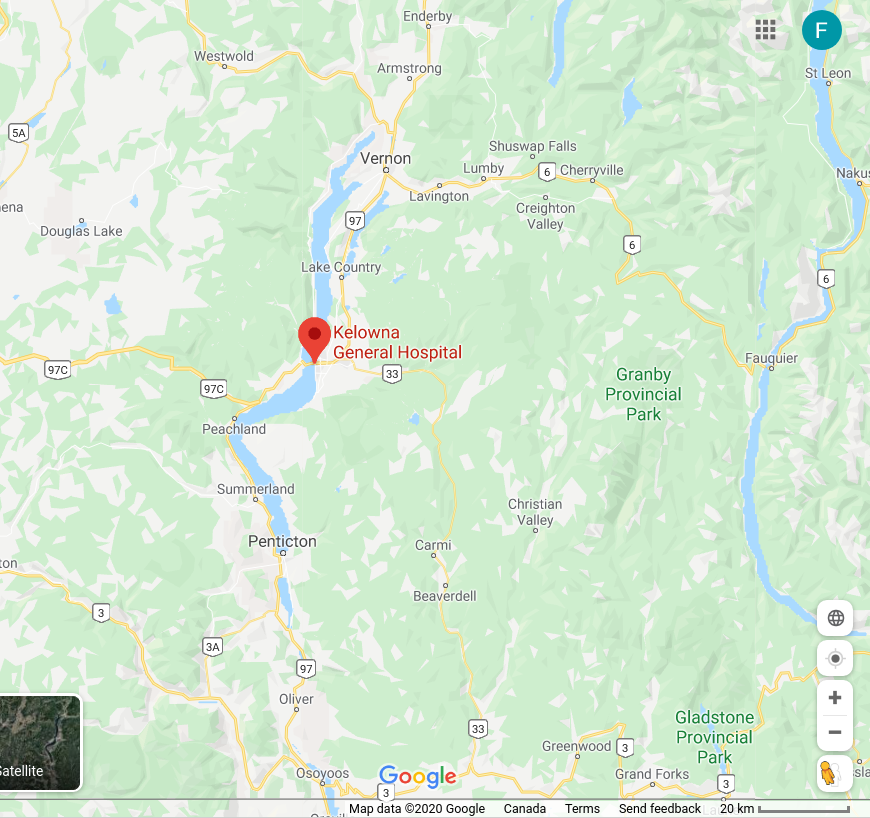
\includegraphics[width=\linewidth]{OkanaganMap.png}
  \caption{A map of the Okenagan Valley showing the location of Kelowna, where the closesed hospital is.}
  \label{fig:OkanMap}
\end{figure}
The feild crew will be based in Kelowna (N49.878761, W -119.511708), where the closesed hospital is (see Figure \ref{fig:OkanMap} ). Feildwork will involve driving to various vinyards within a 30km radius up and down the Okanagan valley. All sites are accesible by well maintained roads. Onece on site, crew members will scope out vinyards and plan which vine plants will be selected for phenological monitoring next year. This activity needs to take place this year because our contacts with teh vinyards are retiring thsi year, and so will be unavailable to facilitate project set up next year. We must set up our feild sites in early May because later in the year the vinyard employees are busy applying various viticultural parctices accros the vinyards. The vinyards will therefore be less amenable after May and the risks of coming into contact with vineyard employees will be higher.   

\subsubsection{Equipment and training }
The main feild vehicle that Faith and Mira will drive has been recently serviced and contains a first aid kit. A printed copy of the lab emergency procedure, emergency contacts, MSP information, and the location of the nearest hospital or clinic will also be stored with the field safety equipment. Crew members will work in a minimum of pairs, while practicing appropiate social distancing measures. They will also carry mobile phones with them, as mobile phone reception is not probematic in the Okenagan Valley, and a first aid kit will be easily accesible in the vehicle on site. All vehicles used for fieldwork will be properly maintained and include equipment such as jumper cables and a spare tire. To avoid fatigue, no driver will drive for long periods without breaks. All drivers are experienced drivers (more than 5 years of experience), and our Principle Investigator ELizabeth Wolkovich has taken both Faith and Mira for road tests prior to the feild trip to ensure that they are safe drivers.  



\section{Identifying and Addressing Specific Health and Safety Concerns}

\subsection{COVID-19}

We are following the principles and guidelines laid out by WorkSafe BC specifically for Forestry field work and COVID-19 safety \url{https://www.worksafebc.com/en/about-us/covid-19-updates/covid-19-industry-information/forestry} 

\subsubsection {Pre-departure Health Screening}
In order to undertake travel to the research site, we will first ensure that crew members are healthy prior to departure. All three crew members will begin Temperature/Symptom Tracking two weeks before the day we are to leave for the field. Temperature screening will be done with a properly calibrated thermometer, with temperature thresholds based on Health Canada guidelines. An indicator for possible COVID-19 infection is 37.5 C. Active daily monitoring will be conducted using the Personal Health Daily Monitoring Form (from the BC Centre for Disease Control). All crew members must complete the form which is provided below. Any crew member that has had a confirmed case of COVID-19 or who is unwell at the time of departure based on the COVID-19 symptoms being tracked using the Personal Health Monitoring Form, will not be allowed to take part in this research project.

\subsubsection{Overview}
The crew consists of three team members. Other than driving to and from the accommodation, and driving to the field sites, all of the work is outdoors, and there will be no difficulty in maintaining appropriate social distancing of two meter minimum distances. Any team meetings will take place outside to maintain physical distance. All team members will be responible for ensuring physical distancing is maintained and any special COVID-19 precautions are strictly followed as per WorkSafe BC guidelines. Good hygine will be practiced at all times, in line with the  WorkSafe BC recomendations.    

\subsubsection{Location}
Faith and Mira will stay in a large apartment in Kelowna. They will have seperate bedrooms and washrooms, and will sanitise communal space and equipment reguarly and remain 2 meters appart at all times. They will also be responsible for their own food preperation and cooking. Elizabeth will stay in a seperate apartment close by. Each crew member will have their own sanitizer and hygiene supplies for personal use for the duration of the field work. There will also be bulk liquid soap, water, and sanitizer that the crew can use to fill their personal containers if the need arises. Elizabeth will be in her own vehicle, while Faith and Mira will share a feild vehicle. In the shared vehicle the passenger in the back-passenger seat will be diagonally positioned relative to the driver to maintain a two meter distance ensuring physical distancing is in place as per WorkSafe BC guidelines. All crew will wash hands with soap and water (or with hand sanitizer) prior to entering the vehicles. The interior (e.g. seatbelts, headrests, door handles, steering wheels, and hand holds) and exterior door handles of both vehicles will be wiped down with sanitizing cleaner at the end of each day, or sooner if a member of the crew reports COVID-19 symptoms.  

\subsubsection{Exhibiting COVID-19 symptoms}
If a crew member exhibits COVID-19 symptoms (e.g. sore throat, fever, sneezing or coughing) they would be put into the far back seat of their truck, and instructed to put on a protective face mask and gloves. The other crew member, if not already the driver, would become the driver and they would put on a protective face mask and gloves. The inside of the vehicle (e.g. seatbelts, headrests, door handles, steering wheels, and hand holds) would then be wiped down with sanitizing cleaner. The vehicle would immediately head back to Vancouver not stopping along the way (we have extra gas in Gerry cans in the truck bed, and food/water). The drive time would be up to but likely not more than 6 hours. During the drive, the person with symptoms would continue to monitor their situation using a thermometer and tracking other health metrics (see Personal Health Daily Monitoring Form below). We have thermometers in the vehicles to enable effective monitoring. The vehicle interior and exterior door handles would be wiped down with sanitizing cleaner upon completion of the drive. Following the protocols set out by WorkSafe BC, both the person with symptoms and the driver would go into self-isolation in their homes for two weeks. The research supervisor would immediately notify the Public Health Authority in British Columbia by dialing 811 that someone with symptoms is self-isolating. We would notify the management of our field accommodation so that they could take necessary cleaning precautions.  Any crew that has had a confirmed case of COVID-19 will not be allowed to come to work.

\subsubsection{Interactions with collaborators}
We will be interacting with local colaborators, but will maintain social distance from then as per the WorkSafe BC recomendations. To this end, all meetings will be kept to a minimum, and will take place outside where there is enough space for 2 meters between every person. We will also paractice good hygine, including wearing face masks, not touching faces, washing hands often and for at least 20 seconds (or sanitising hands if washing not possible) and sneesing/couphing into disposable tissues if needed. 

\subsubsection{Interactions with field workers in vineyards}
We will alert vinyards to our presence on site so we and feild workers will be aware of each other's presence. Our feildwork does not require interaction with such workers, so if we see any workers we will retreat to a safe distance until they have left the immediate area. Any surfaces we and vinyard feildworkers might come into conact with will be sanitised before and after contact. Our own crew members will also maintain a 2 meter distance from each other at all times as per the WorkSafe BC guidelines.   

\subsubsection{Interactions with local communities}
Our feild base will be close to the town of Kelnowa, where we plan to obtain necisary groceries and gass. To reduce risk to local communities, we will keep shoping trips to a minimum (once a week), wear face masks, and sanitise our hands before and after shoping, and maintaing good hygine. We will only use self-service gass stations and prior to use we will wipe down the gas pump nozzle and PIN pad on the pump with sanitizing wipes. We will not come into contact with any First Nation communities in the Okenagan Valley. 


\end{document}

The fieldwork in the Okanagan should be OK as long as your crew is small, there are no more than two people in a vehicle together, one driving and one in the back right seat (unless from the same household), social distancing can be maintained while working and in accommodations (unless from the same household), and there is no contact with indigenous communities. I've attached a few exemptions that have been approved, and here's a useful link to the WorkSafe BC recommended safety practices for forestry fieldwork that has largely been adopted by some of the other applications (Simard and Hinch). https://www.worksafebc.com/en/about-us/covid-19-updates/covid-19-industry-information/forestry I know working in a vineyard and in a remote field site are different, but there are still transportation, social distancing, PPE and sanitation concerns. You will also need to address how you will interact with or avoid farm workers at these sites. I would also say that you should be able to get the plots set up, but should defer any data collection that can wait for next year.